\chapter{Cơ sở lý thuyết và các nghiên cứu liên quan}
\label{ch:co-so-ly-thuyet}

Chương này trình bày cơ sở lý thuyết y sinh học và phương pháp luận học máy nền tảng cho bài toán dự đoán mức độ triệu chứng trầm cảm từ dữ liệu sinh lý dạng bảng, đồng thời khảo sát có hệ thống các công trình nghiên cứu tiền nhiệm. Nội dung chương tập trung vào: (1) Cấu trúc thang đo chuẩn PHQ-9 và các cơ chế sinh học kết nối chỉ số cận lâm sàng với triệu chứng trầm cảm; (2) Hai thách thức bản chất của dữ liệu y tế dạng bảng gồm mất cân bằng lớp cực đoan và chồng lấn phân phối đặc trưng; (3) Ba trường phái mô hình hóa gồm phân loại phẳng, phân loại phân cấp kết hợp lý thuyết quyết định nhạy chi phí Bayes, và phân loại thứ bậc; (4) Tổng hợp các nghiên cứu liên quan nhằm định vị rõ khoảng trống học thuật mà đề tài giải quyết.

\section{Thang đo PHQ-9 và cơ sở sinh lý học của triệu chứng trầm cảm}
\label{sec:thang-do-phq9-va-sinh-ly}

\subsection{Cấu trúc thang đo PHQ-9 và lượng hóa lâm sàng}
\label{subsec:cau-truc-phq9}

Thang đo Sức khỏe Bệnh nhân 9 mục (Patient Health Questionnaire-9 -- PHQ-9) là một cấu phần chẩn đoán tâm thần tiêu chuẩn hóa, do Kroenke, Spitzer và Williams phát triển \cite{kroenke2001phq, spitzer1999validation}. PHQ-9 gồm 9 mục tự báo cáo phản ánh tần suất xuất hiện các triệu chứng trong vòng hai tuần gần nhất, tương ứng với tiêu chuẩn DSM-IV: (1) Giảm sự hứng thú hoặc niềm vui trong các hoạt động; (2) Cảm giác buồn bã, chán nản hoặc tuyệt vọng; (3) Rối loạn giấc ngủ; (4) Mệt mỏi, thiếu năng lượng; (5) Rối loạn cảm giác thèm ăn; (6) Cảm giác tự ti hoặc mặc cảm tội lỗi; (7) Giảm khả năng tập trung; (8) Chậm chạp vận động hoặc bồn chồn; (9) Ý nghĩ về cái chết hoặc tự làm hại bản thân.

Mỗi mục được chấm điểm theo thang Likert 4 mức độ từ 0 đến 3 (0: Hoàn toàn không; 1: Vài ngày; 2: Hơn một nửa số ngày; 3: Gần như mỗi ngày). Tổng điểm số $s = \sum_{j=1}^9 \text{DPQ}_j \in [0, 27]$ được ánh xạ thành 5 mức độ nghiêm trọng lâm sàng chuẩn được minh họa trong Hình \ref{fig:phq9-tiers}.

\begin{figure}[htbp]{Thang đo PHQ-9 (0--27 điểm), 5 bậc nghiêm trọng lâm sàng và ánh xạ sang không gian 3 nhóm $T_3$}
\centering
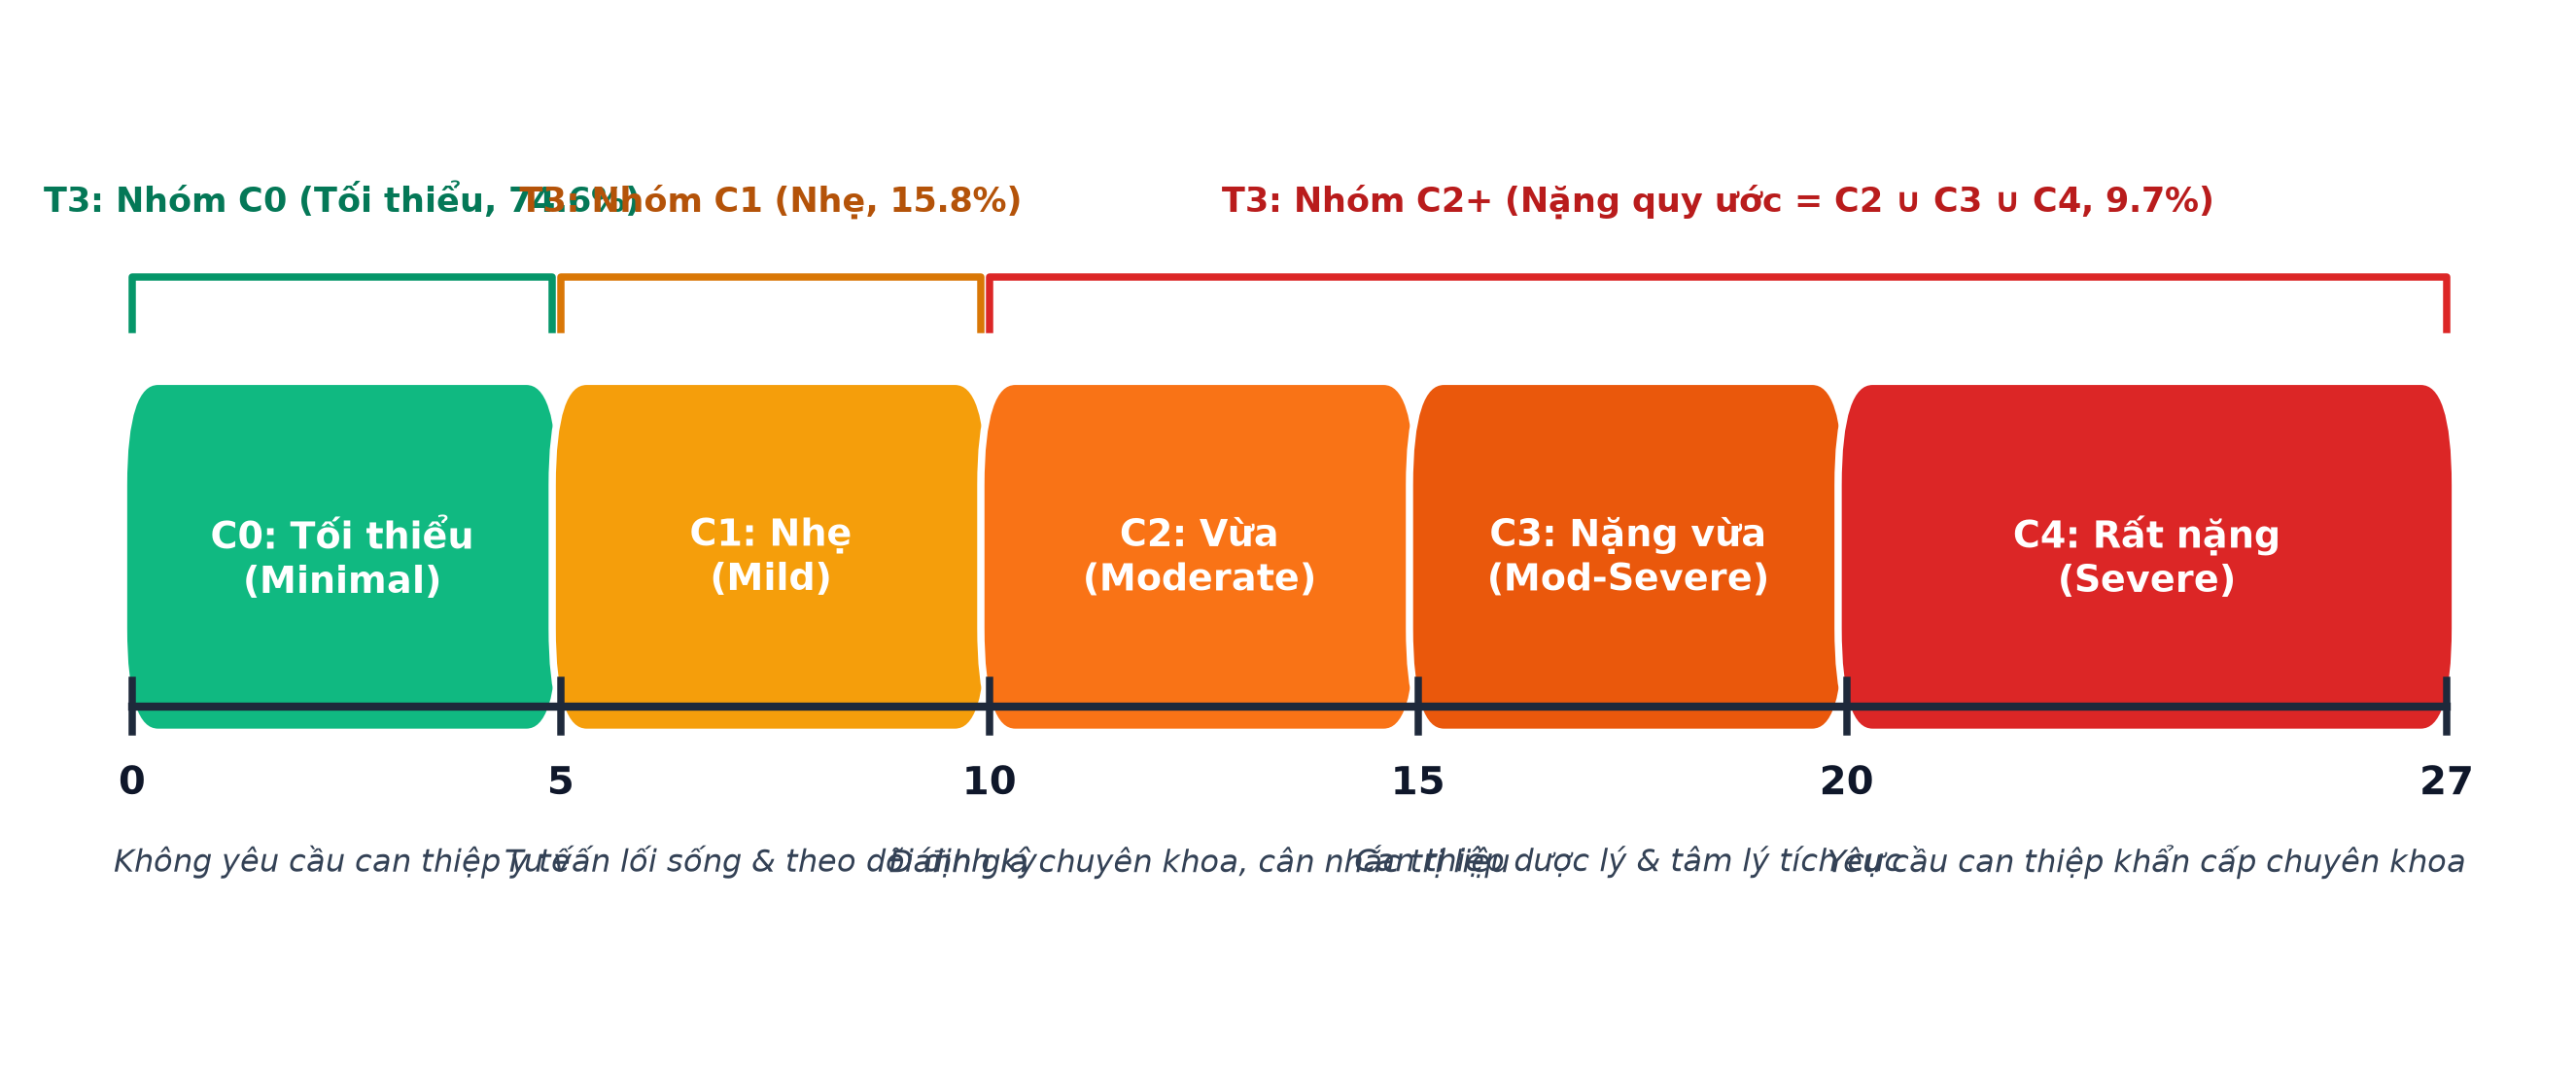
\includegraphics[width=\textwidth]{figures/fig2_phq9_tiers.png}
\label{fig:phq9-tiers}
\end{figure}
\FloatBarrier

Theo quy ước quốc tế:
\begin{itemize}
    \item $s \in [0, 4]$ ($C_0$ -- Tối thiểu): Trạng thái bình thường, không yêu cầu can thiệp y tế.
    \item $s \in [5, 9]$ ($C_1$ -- Nhẹ): Xuất hiện triệu chứng cận lâm sàng, khuyến nghị theo dõi và tư vấn tâm lý lối sống.
    \item $s \in [10, 14]$ ($C_2$ -- Vừa): Ngưỡng cắt lâm sàng bắt đầu điều trị, cần bác sĩ chuyên khoa đánh giá.
    \item $s \in [15, 19]$ ($C_3$ -- Nặng vừa): Cần can thiệp tích cực kết hợp liệu pháp dược lý và tâm lý.
    \item $s \in [20, 27]$ ($C_4$ -- Rất nặng): Yêu cầu can thiệp khẩn cấp chuyên khoa tâm thần.
\end{itemize}

Trong khuôn khổ đề tài DepSev-ML, bên cạnh không gian 5 bậc tiêu chuẩn ($T_5$), bài toán còn được khảo sát trên không gian 3 nhóm gộp quy ước ($T_3$), trong đó nhóm $C_2^+$ đại diện cho toàn bộ các đối tượng có triệu chứng từ mức Vừa đến Rất nặng ($C_2 \cup C_3 \cup C_4$, tương ứng $s \ge 10$).

\subsection{Cơ sở sinh lý học và các chỉ dấu y sinh học}
\label{subsec:co-so-sinh-ly}

Mặc dù triệu chứng trầm cảm thể hiện qua cảm xúc và hành vi, các nghiên cứu y sinh học hiện đại đã chứng minh trầm cảm là một bệnh lý toàn thân có tương tác mật thiết với các rối loạn sinh hóa và chuyển hóa ngoại vi thông qua trục não-ruột, hệ thống miễn dịch và trục hạ đồi-tuyến yên-tuyến thượng thận (HPA) \cite{pratt1991discriminant}.

\begin{figure}[htbp]{Các cơ chế y sinh học liên kết chỉ số sinh lý ngoại vi với mức độ triệu chứng trầm cảm}
\centering
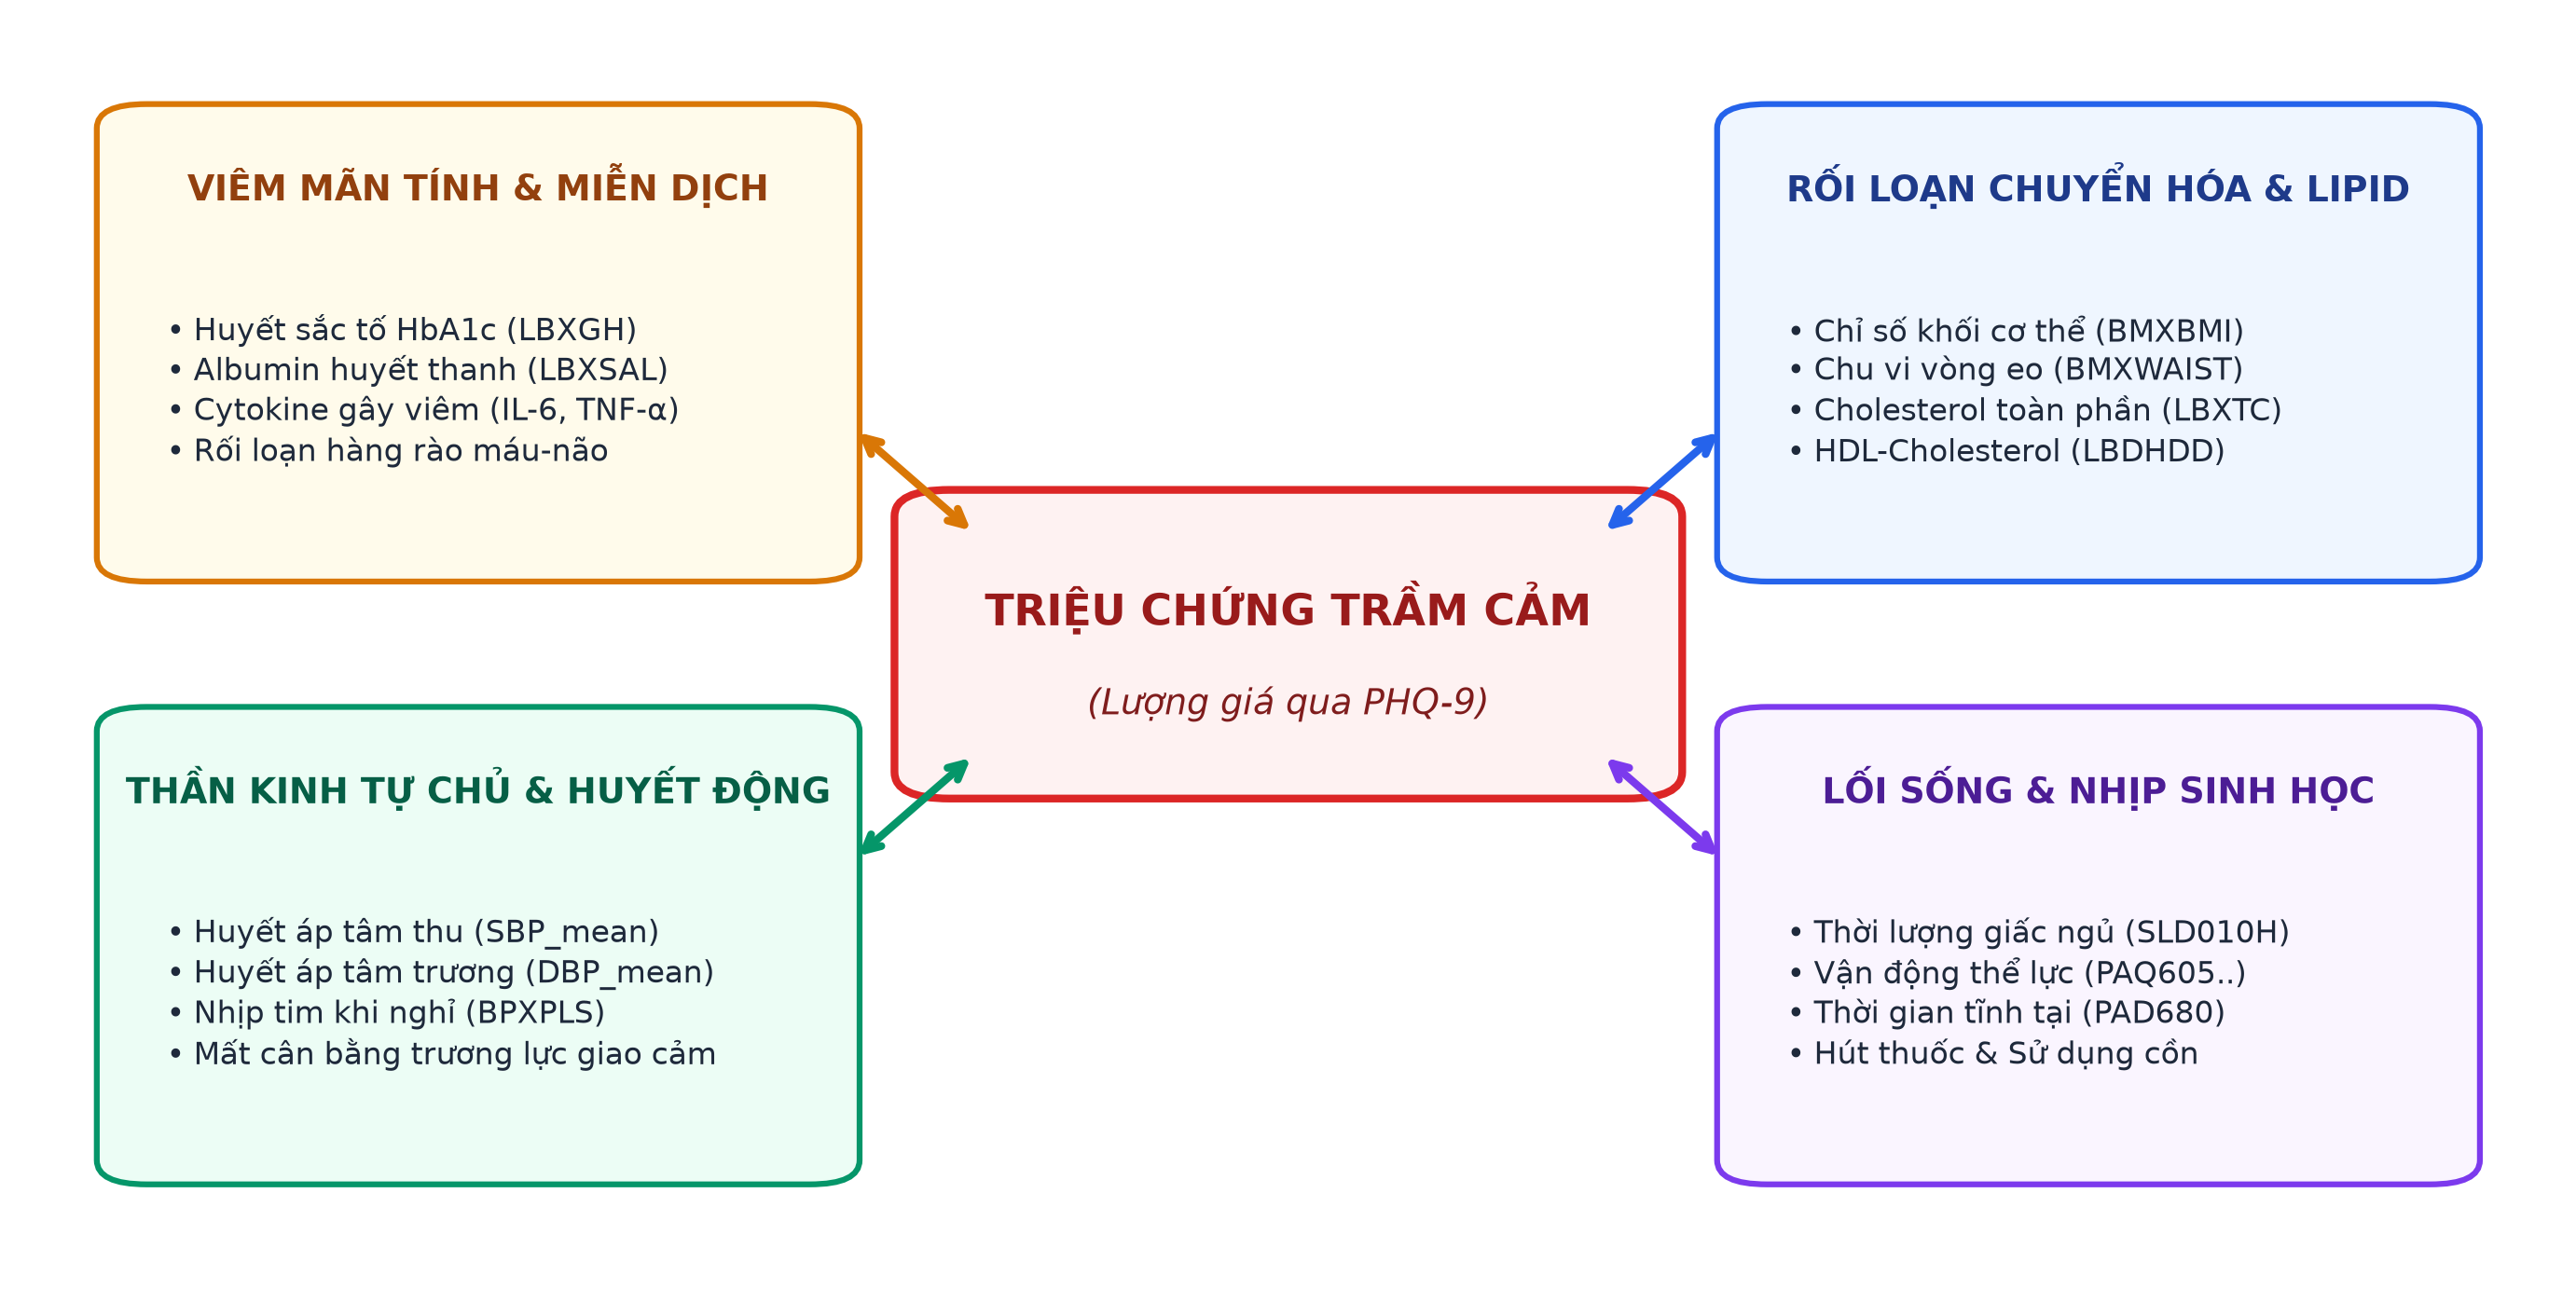
\includegraphics[width=\textwidth]{figures/fig2_gut_brain_metabolic_axis.png}
\label{fig:gut-brain-axis}
\end{figure}
\FloatBarrier

Như mô tả trong Hình \ref{fig:gut-brain-axis}, các nhóm biến số ngoại vi trong NHANES phản ánh bốn cơ chế bệnh sinh chính:
\begin{enumerate}
    \item \textbf{Phản ứng viêm mãn tính thể nhẹ và miễn dịch ngoại vi:} Trầm cảm kích hoạt các cytokine gây viêm ngoại vi (IL-6, TNF-$\alpha$). Nồng độ Albumin huyết thanh (LBXSAL) phản ánh tình trạng dinh dưỡng và là protein điều biến phản ứng viêm âm tính; trong khi chỉ số đường huyết tích lũy Glycohemoglobin HbA1c (LBXGH) phản ánh mức độ căng thẳng oxy hóa và kháng insulin.
    \item \textbf{Rối loạn chuyển hóa và lipid huyết tương:} Sự rối loạn hoạt động chuyển hóa thể hiện rõ qua các chỉ số nhân trắc học như chỉ số khối cơ thể (BMXBMI), chu vi vòng eo (BMXWAIST), kết hợp cùng nồng độ Cholesterol toàn phần (LBXTC) và HDL-Cholesterol bảo vệ tim mạch (LBDHDD).
    \item \textbf{Hệ thần kinh tự chủ và huyết động học:} Sự mất cân bằng giữa trương lực giao cảm và phó giao cảm dẫn đến biến đổi nhịp tim khi nghỉ (BPXPLS), huyết áp tâm thu (SBP\_mean) và huyết áp tâm trương (DBP\_mean).
    \item \textbf{Hành vi lối sống và nhịp sinh học:} Giấc ngủ suy giảm (SLD010H), mức độ hoạt động thể lực thấp, thời gian ngồi tĩnh tại kéo dài (PAD680) cùng với hành vi sử dụng chất kích thích (hút thuốc, rượu bia) có mối quan hệ nhân quả hai chiều với sự gia tăng triệu chứng trầm cảm.
\end{enumerate}

\section{Đặc thù và thách thức của dữ liệu y tế dạng bảng}
\label{sec:dac-thu-du-lieu-bang}

Dữ liệu y tế dạng bảng trích xuất từ các khảo sát cộng đồng như NHANES có những đặc thù hình học phức tạp, khác biệt căn bản so với dữ liệu hình ảnh hay văn bản.

\subsection{Mất cân bằng lớp cực đoan (Severe Class Imbalance)}
\label{subsec:mat-can-bang-lop}

Trong các cuộc điều tra dịch tễ quy mô quốc gia, tỷ lệ mắc các bệnh lý tâm thần mức độ nghiêm trọng luôn chiếm thiểu số. Tỷ số mất cân bằng (Imbalance Ratio -- IR) được định nghĩa bởi:
\begin{equation}
    \text{IR} = \frac{\max_k N_k}{\min_k N_k}
\end{equation}
Trong tập dữ liệu phát triển Legacy của đề tài ($N = 4.045$), lớp $C_0$ chiếm tới $3.016$ đối tượng (74.56\%), trong khi lớp rất nặng $C_4$ chỉ có $44$ đối tượng (1.09\%), tạo nên tỷ số mất cân bằng lên tới $\text{IR} = 3016 / 44 \approx 68.5:1$ (Hình \ref{fig:imbalance-overlap}a).

Nếu mô hình học máy được huấn luyện nhằm tối thiểu hóa sai số toàn cục thông thường, thuật toán sẽ bị thiên lệch mạnh về phía lớp $C_0$, dẫn tới hiện tượng đạt độ chính xác Accuracy rất cao nhưng hoàn toàn bỏ sót các ca bệnh thực tế. Để khắc phục hiện tượng này, kỹ thuật gán trọng số nghịch đảo tần số lớp (Class-weighted objective) được áp dụng:
\begin{equation}
    w_k = \frac{N}{K \cdot N_k}
\end{equation}
giúp cân bằng lại đóng góp của các mẫu thuộc lớp hiếm vào quá trình tối ưu hóa.

\begin{figure}[htbp]{(a) Mất cân bằng lớp cực đoan trên tập dữ liệu và (b) Hiện tượng chồng lấn phân phối đặc trưng sinh lý}
\centering
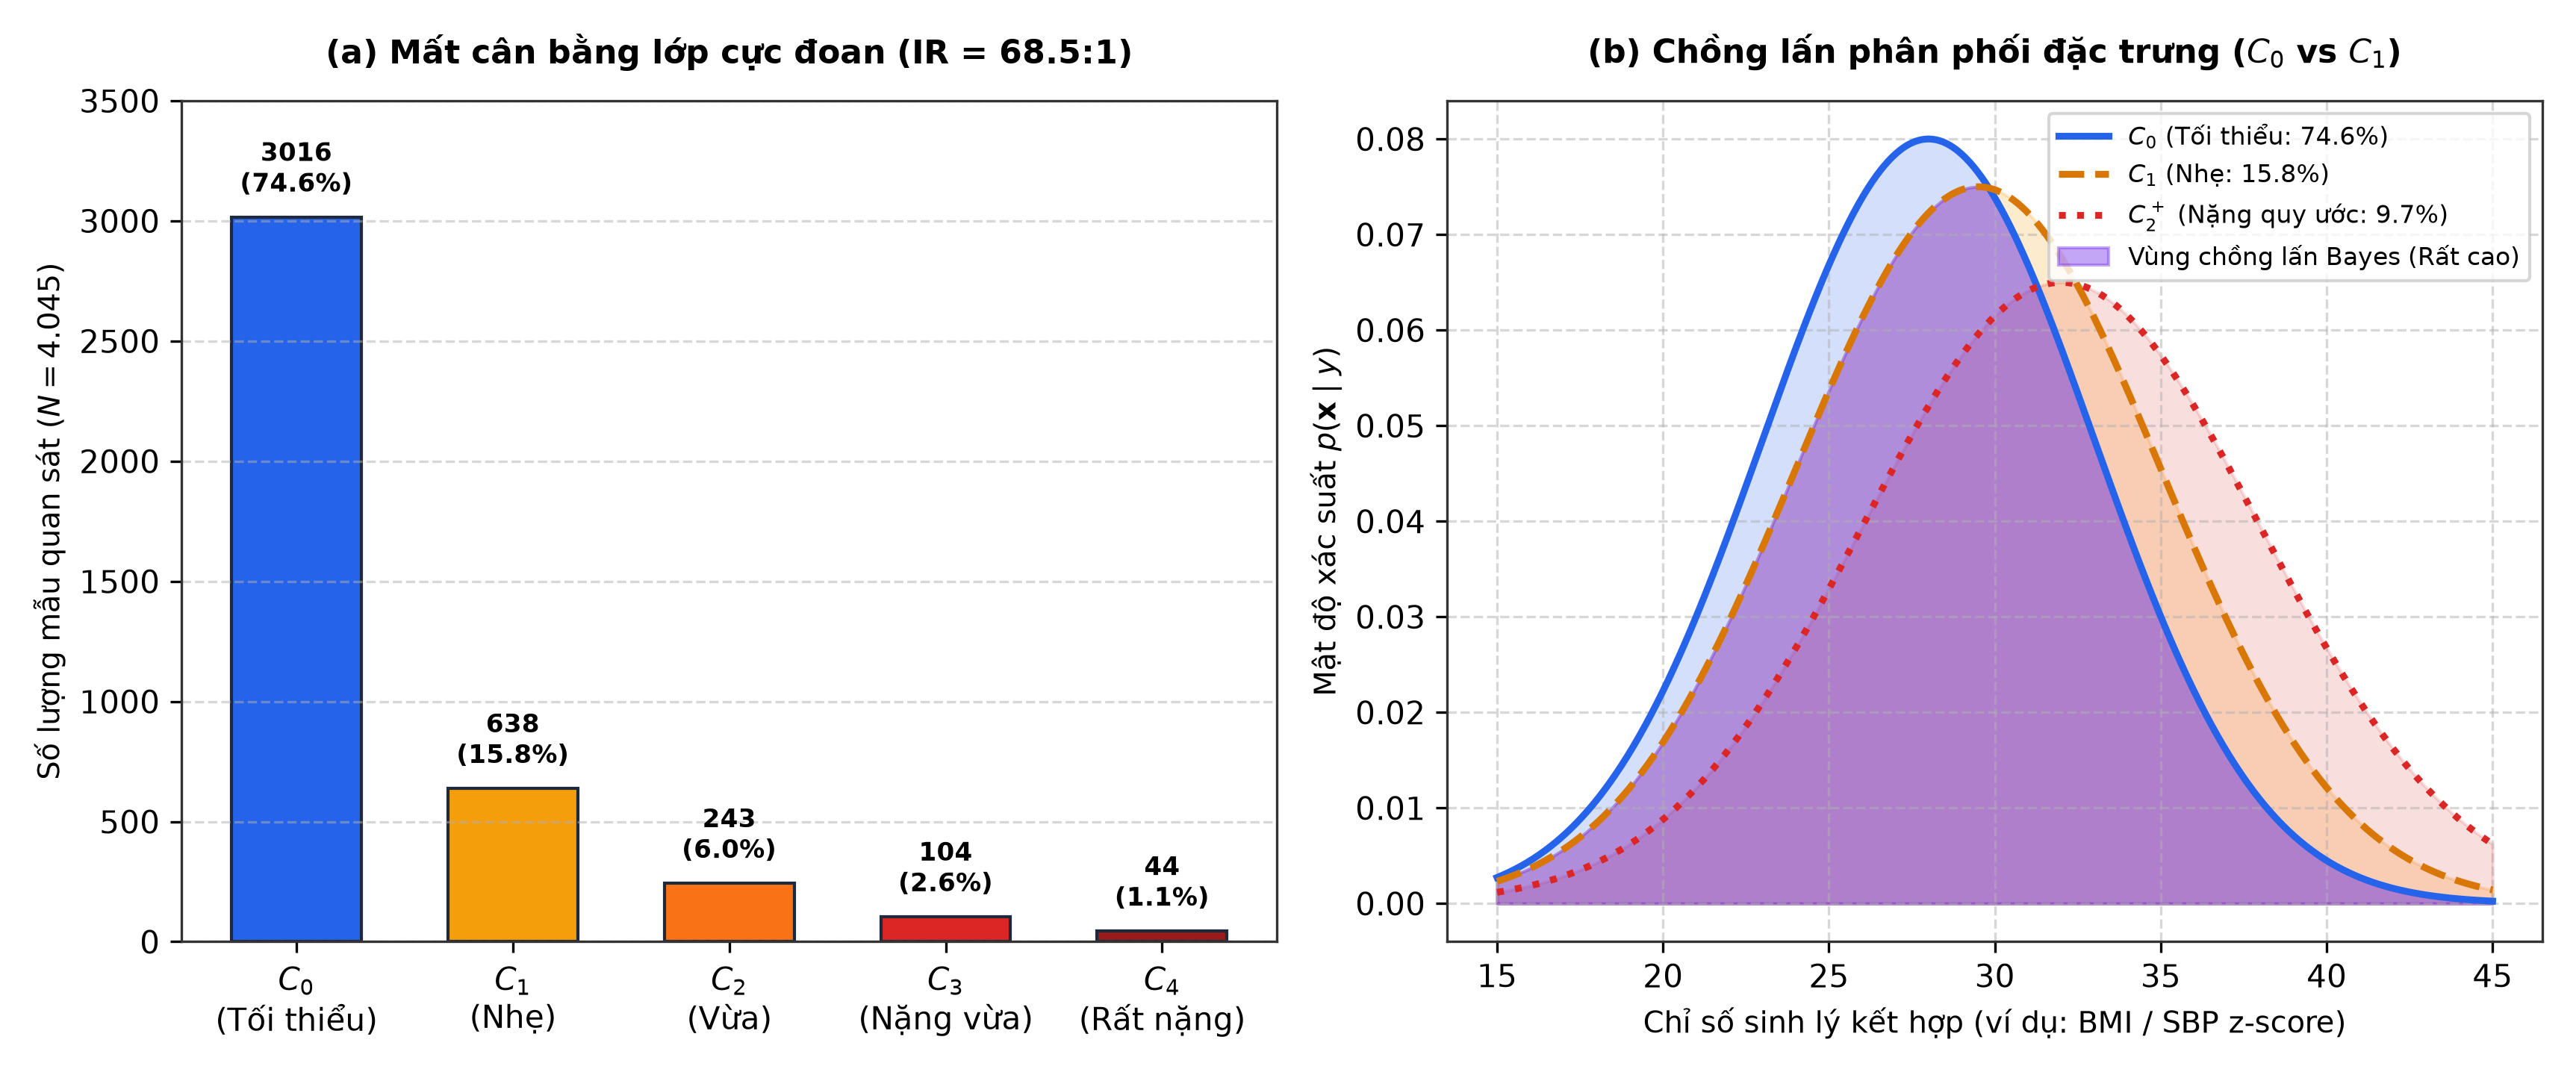
\includegraphics[width=\textwidth]{figures/fig2_imbalance_overlap.png}
\label{fig:imbalance-overlap}
\end{figure}
\FloatBarrier

\subsection{Chồng lấn phân phối đặc trưng (Feature Overlap)}
\label{subsec:chong-lan-dac-trung}

Khác với các xét nghiệm chẩn đoán đặc hiệu, các chỉ số sinh lý như huyết áp, cholesterol hay BMI không có một ngưỡng cắt sinh học duy nhất để phân tách người bình thường và người có triệu chứng trầm cảm. Phân phối xác suất điều kiện của đặc trưng $\mathbf{x}$ giữa hai trạng thái kế cận $p(\mathbf{x} \mid Y = 0)$ và $p(\mathbf{x} \mid Y = 1)$ có diện tích giao thoa rất lớn (Hình \ref{fig:imbalance-overlap}b).

Khi vùng giao thoa phân phối sinh lý giữa các lớp lớn, bộ phân loại không thể đạt được độ chính xác phân tách tuyệt đối nếu không bổ sung chiều thông tin đặc hiệu mới. Do đó, việc cải thiện hiệu năng đòi hỏi phải khai thác các kiến trúc phân loại phù hợp và kiểm soát chặt chẽ sự đánh đổi lâm sàng.

\section{Khảo sát các thuật toán học máy và Cơ sở lý thuyết Rừng ngẫu nhiên}
\label{sec:cac-thuat-toan-va-rf}

\subsection{Khảo sát ngắn gọn các thuật toán học máy cơ sở và Lý do lựa chọn Rừng ngẫu nhiên}
\label{subsec:khao-sat-thuat-toan-co-so}

Để giải quyết bài toán phân loại mức độ triệu chứng trầm cảm trên dữ liệu y tế dạng bảng NHANES, nghiên cứu đã thử nghiệm 4 thuật toán học máy tiêu biểu thuộc các họ phương pháp khác nhau nhằm xây dựng và đánh giá các mô hình cơ sở (baselines):
\begin{itemize}
    \item \textbf{Hồi quy Logistic (Logistic Regression):} Mô hình tuyến tính kinh điển trong nghiên cứu dịch tễ học và y học chứng cứ, ước lượng xác suất hậu nghiệm thông qua hàm Sigmoid/Softmax, có ưu điểm tính toán nhanh, tính ổn định cao và khả năng suy diễn tỷ số chênh (Odds Ratio) rõ ràng.
    \item \textbf{Cây quyết định (Decision Tree):} Mô hình phi tuyến dựa trên các quy tắc logic rẽ nhánh nhị phân trực quan kiểu \texttt{IF-THEN}, không đòi hỏi chuẩn hóa thang đo biến số nhưng có phương sai lớn và cực kỳ nhạy cảm với biến động dữ liệu.
    \item \textbf{Rừng ngẫu nhiên (Random Forest):} Phương pháp học kết hợp theo cơ chế đóng bao (Bagging) và ngẫu nhiên hóa đặc trưng, tập hợp nhiều cây quyết định độc lập nhằm triệt tiêu phương sai và chống quá khớp vượt trội.
    \item \textbf{Tăng cường độ dốc cực đại (XGBoost):} Phương pháp học kết hợp tăng cường (Gradient Boosting) xây dựng quần thể cây tuần tự nhằm bù trừ phần dư của hàm mất mát, có năng lực khớp hàm phi tuyến mạnh mẽ.
\end{itemize}

Các thuật toán trên được triển khai đồng nhất trên cùng một giao thức kiểm định lồng nhau (Nested Cross-Validation, chi tiết tại Chương \ref{ch:thuc-nghiem}). Bảng \ref{tab:nested-cv-comparison} (Mục \ref{sec:tuning-va-ensemble}) tổng hợp đầy đủ kết quả so sánh đối chuẩn khách quan giữa các thuật toán.

\textbf{Lý do lựa chọn Rừng ngẫu nhiên làm mô hình cơ sở chính:} Dựa trên kết quả thực nghiệm thực tế từ Nested CV trên không gian 34 đặc trưng đầy đủ ($F_4$), Rừng ngẫu nhiên đạt chỉ số Macro-F1 trung bình cao nhất trong nhóm các mô hình phẳng được khảo sát ($0.2755 \pm 0.0270$) và Weighted-F1 đạt $0.6437 \pm 0.0087$, tạo mức cải thiện vượt bậc $+0.0523$ so với cấu hình mặc định ban đầu ($0.2232$). 

Quyết định lựa chọn Random Forest được đưa ra trên cơ sở thực tế và khiêm tốn: mô hình không khẳng định dẫn đầu tuyệt đối trên mọi chỉ số đơn lẻ (chẳng hạn Hồi quy Logistic đạt Balanced Accuracy $0.3253$ nhỉnh hơn ở một số ngưỡng do tính trơn của siêu phẳng quyết định, trong khi XGBoost đạt Macro-F1 $0.2621$), song Random Forest mang lại sự cân bằng tốt nhất giữa khả năng nắm bắt quan hệ phi tuyến phức tạp, khả năng chống chịu nhiễu và độ bền vững phương sai trên dữ liệu y tế dạng bảng. Do đó, nghiên cứu lựa chọn Random Forest làm mô hình cơ sở xương sống (Backbone Model) để phân tích chuyên sâu và làm nền tảng cho các kiến trúc tiếp theo.

\subsection{Cấu trúc nền tảng: Nguyên lý hoạt động của Cây quyết định (Decision Tree)}
\label{subsec:decision-tree-theory}

Để hiểu rõ bản chất của Rừng ngẫu nhiên, trước hết cần nắm vững cách một Cây quyết định (Decision Tree) đơn lẻ hoạt động. Cây quyết định là giải thuật phi tham số phân tách đệ quy không gian đặc trưng đa chiều thành các siêu hình hộp chữ nhật trực giao (Hình \ref{fig:dt-concept}).

\begin{figure}[htbp]{Sơ đồ nguyên lý phân nhánh của Cây quyết định trên không gian đặc trưng dạng bảng}
\centering
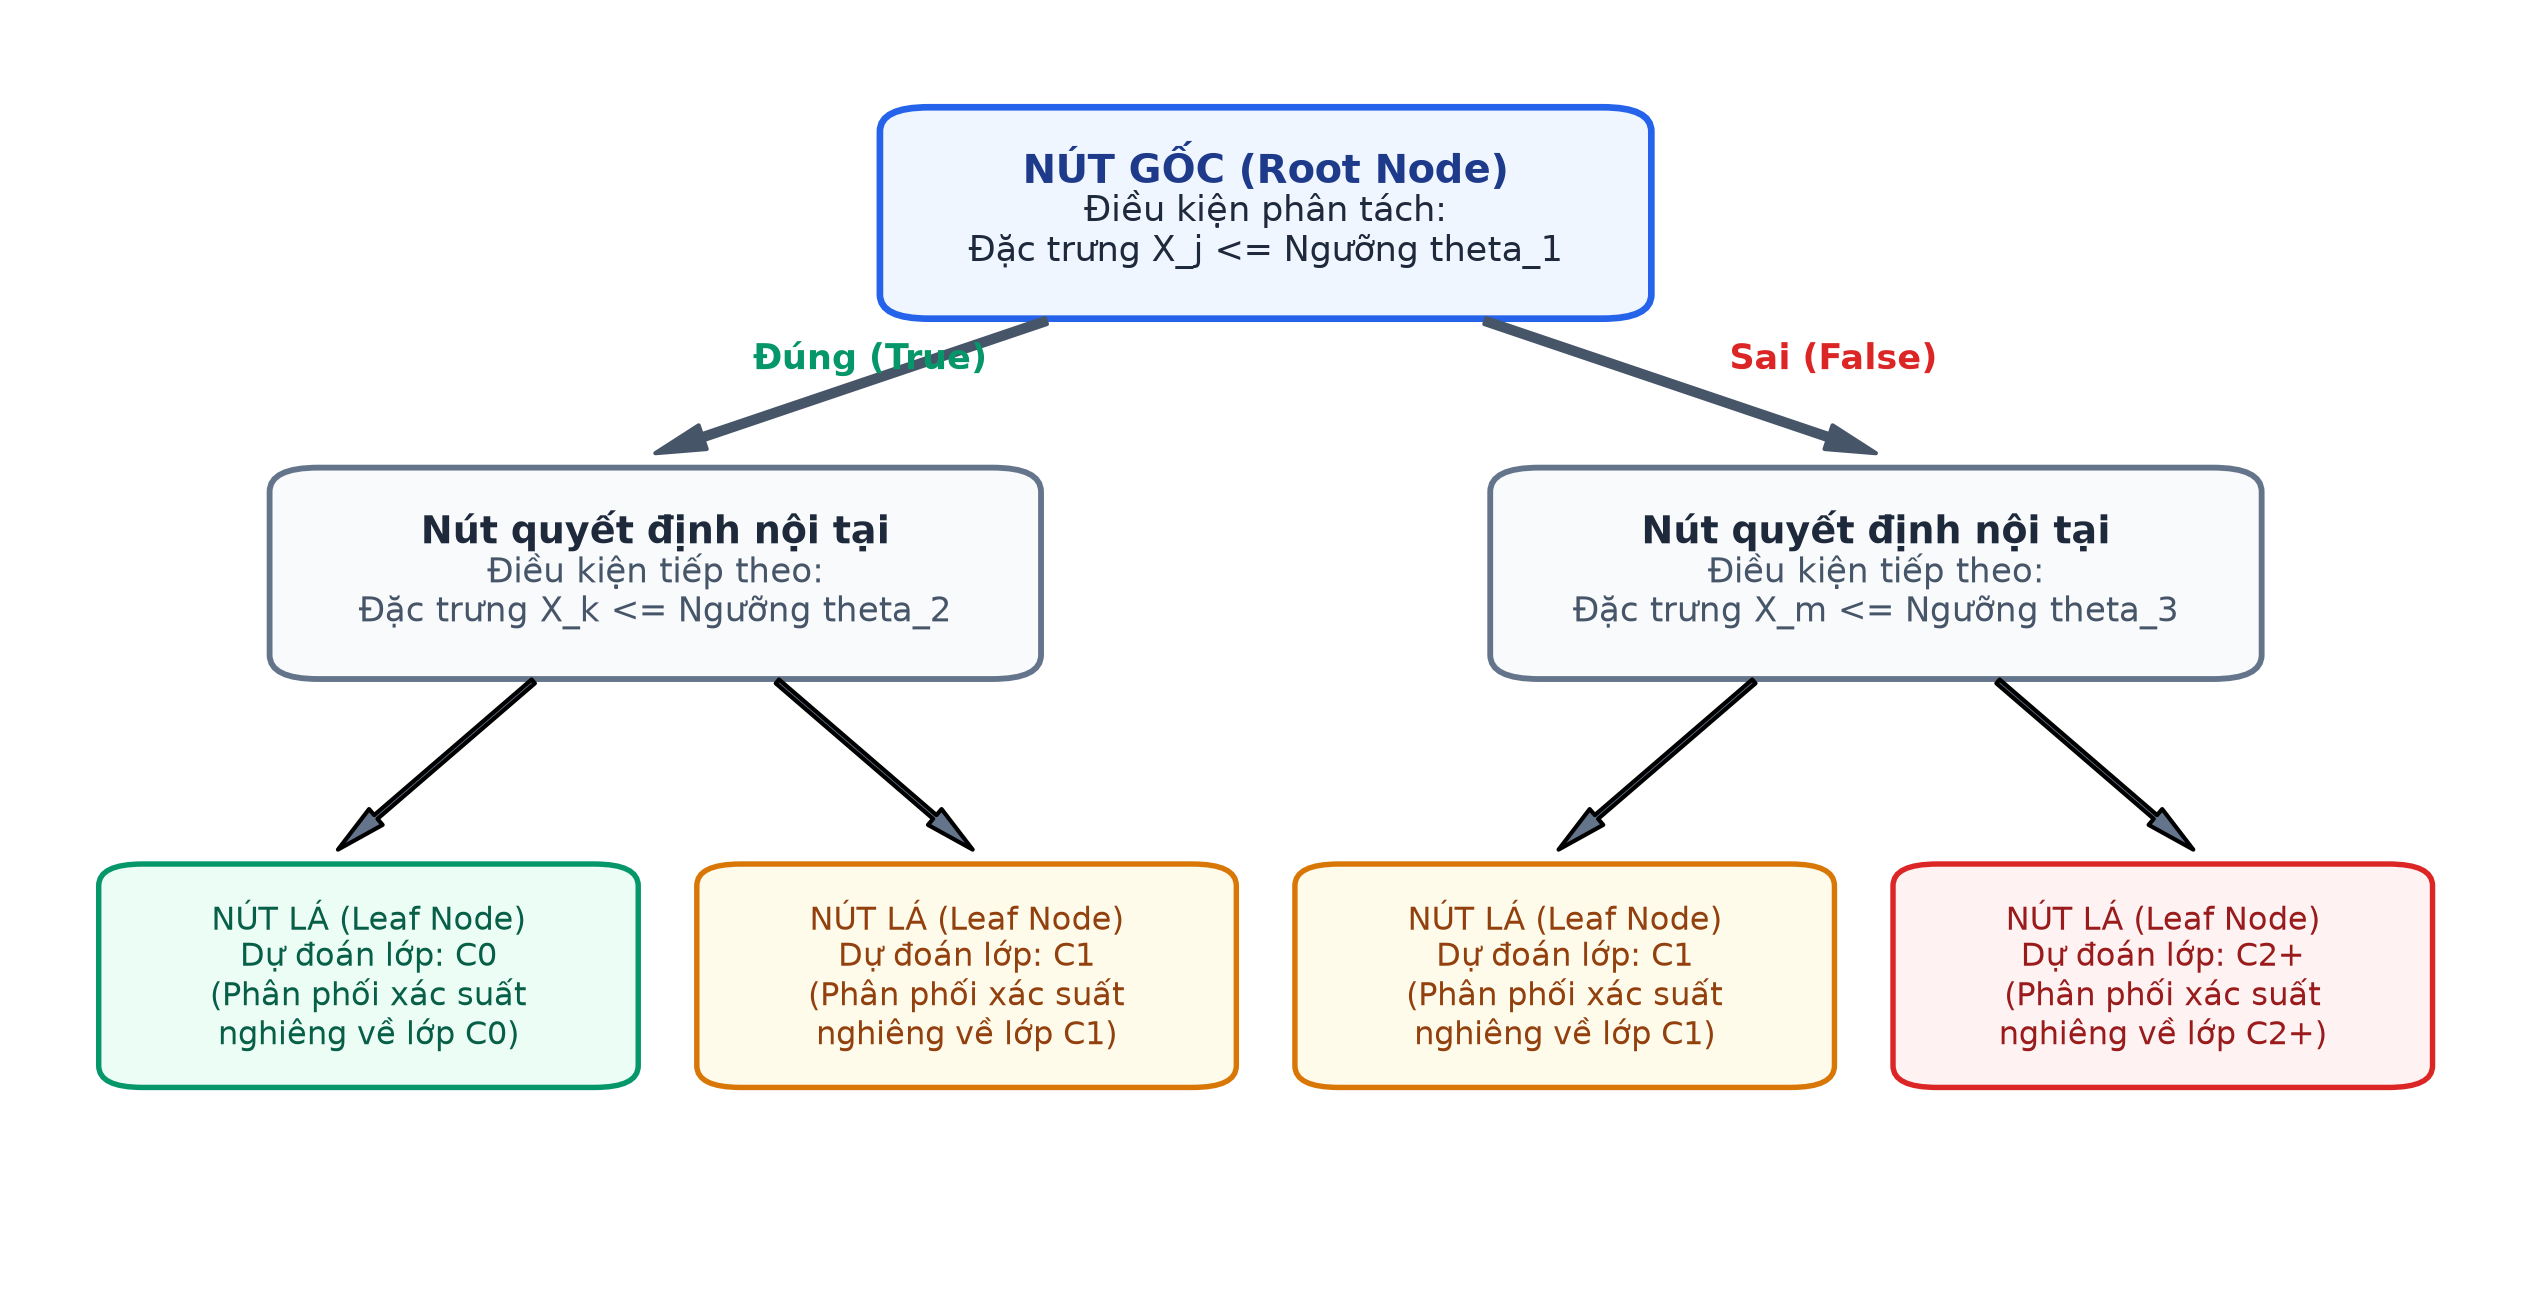
\includegraphics[width=0.88\textwidth]{figures/fig2_decision_tree_concept.png}
\label{fig:dt-concept}
\end{figure}
\FloatBarrier

Quá trình hoạt động của Cây quyết định gồm các nguyên lý cốt lõi:
\begin{enumerate}
    \item \textbf{Cấu trúc phân cấp:} Cây bắt đầu từ một nút gốc (Root Node) chứa toàn bộ tập dữ liệu, phân nhánh qua các nút quyết định nội tại (Internal Decision Nodes) và kết thúc tại các nút lá (Leaf Nodes).
    \item \textbf{Quy tắc phân tách nhị phân:} Tại mỗi nút nội tại, thuật toán duyệt qua các đặc trưng và tìm kiếm một ngưỡng cắt tối ưu $\theta$ đối với đặc trưng $X_j$. Điều kiện $X_j \le \theta$ phân chia tập dữ liệu tại nút thành hai nhánh con: nhánh Đúng (True) và nhánh Sai (False).
    \item \textbf{Tiêu chí tối ưu độ bất thuần (Impurity Criterion):} Việc lựa chọn cặp đặc trưng và ngưỡng cắt $(X_j, \theta)$ tối ưu dựa trên việc tối đa hóa mức giảm độ bất thuần sau phân tách. Trong bài toán phân loại, chỉ số bất thuần Gini (Gini Impurity) được sử dụng phổ biến:
    \begin{equation}
        G = 1 - \sum_{k=0}^{K-1} p_k^2
    \end{equation}
    trong đó $p_k$ là tỷ lệ mẫu thuộc lớp $k$ tại nút đang xét. Nút có $G = 0$ là nút hoàn toàn thuần khiết (chỉ chứa mẫu của một lớp duy nhất).
    \item \textbf{Gán nhãn tại nút lá:} Khi quá trình phân nhánh đạt tiêu chí dừng (độ sâu tối đa, số lượng mẫu tối thiểu tại lá), nút đó trở thành nút lá. Xác suất gán cho từng lớp tại lá chính là tỷ lệ phân bố thực tế của các lớp mẫu rơi vào vùng không gian con đó.
\end{enumerate}

\textbf{Hạn chế căn bản của một Cây quyết định đơn lẻ:} Mặc dù cấu trúc cây hoàn toàn trong suốt và dễ diễn giải dưới dạng các quy tắc \texttt{IF-THEN}, một cây đơn lẻ có \textbf{phương sai cực kỳ cao (high variance)}. Do cấu trúc cây được xây dựng tham lam từ trên xuống dưới, chỉ một biến động nhỏ trong tập dữ liệu huấn luyện (chẳng hạn vài mẫu ngoại lai) cũng có thể làm thay đổi hoàn toàn đặc trưng được chọn ở nút gốc, dẫn đến cấu trúc toàn bộ các tầng cây bên dưới bị biến dạng. Hiện tượng này đặc biệt nghiêm trọng trên dữ liệu y tế thực tế có độ nhiễu cao và mất cân bằng lớp lớn, khiến cây đơn lẻ rất dễ rơi vào tình trạng quá khớp (overfitting).

\subsection{Nguyên lý Rừng ngẫu nhiên và Cơ chế kết hợp nhiều cây}
\label{subsec:random-forest-deepdive}

Rừng ngẫu nhiên (Random Forest) do Leo Breiman đề xuất năm 2001 \cite{breiman2001random} là phương pháp học kết hợp (Ensemble Learning) giải quyết triệt để nhược điểm phương sai cao của cây đơn lẻ bằng cách xây dựng một quần thể gồm $B$ cây quyết định độc lập (Hình \ref{fig:rf-concept}).

\begin{figure}[htbp]{Kiến trúc Rừng ngẫu nhiên: Lấy mẫu Bootstrap, ngẫu nhiên hóa đặc trưng và tổng hợp Soft Voting}
\centering
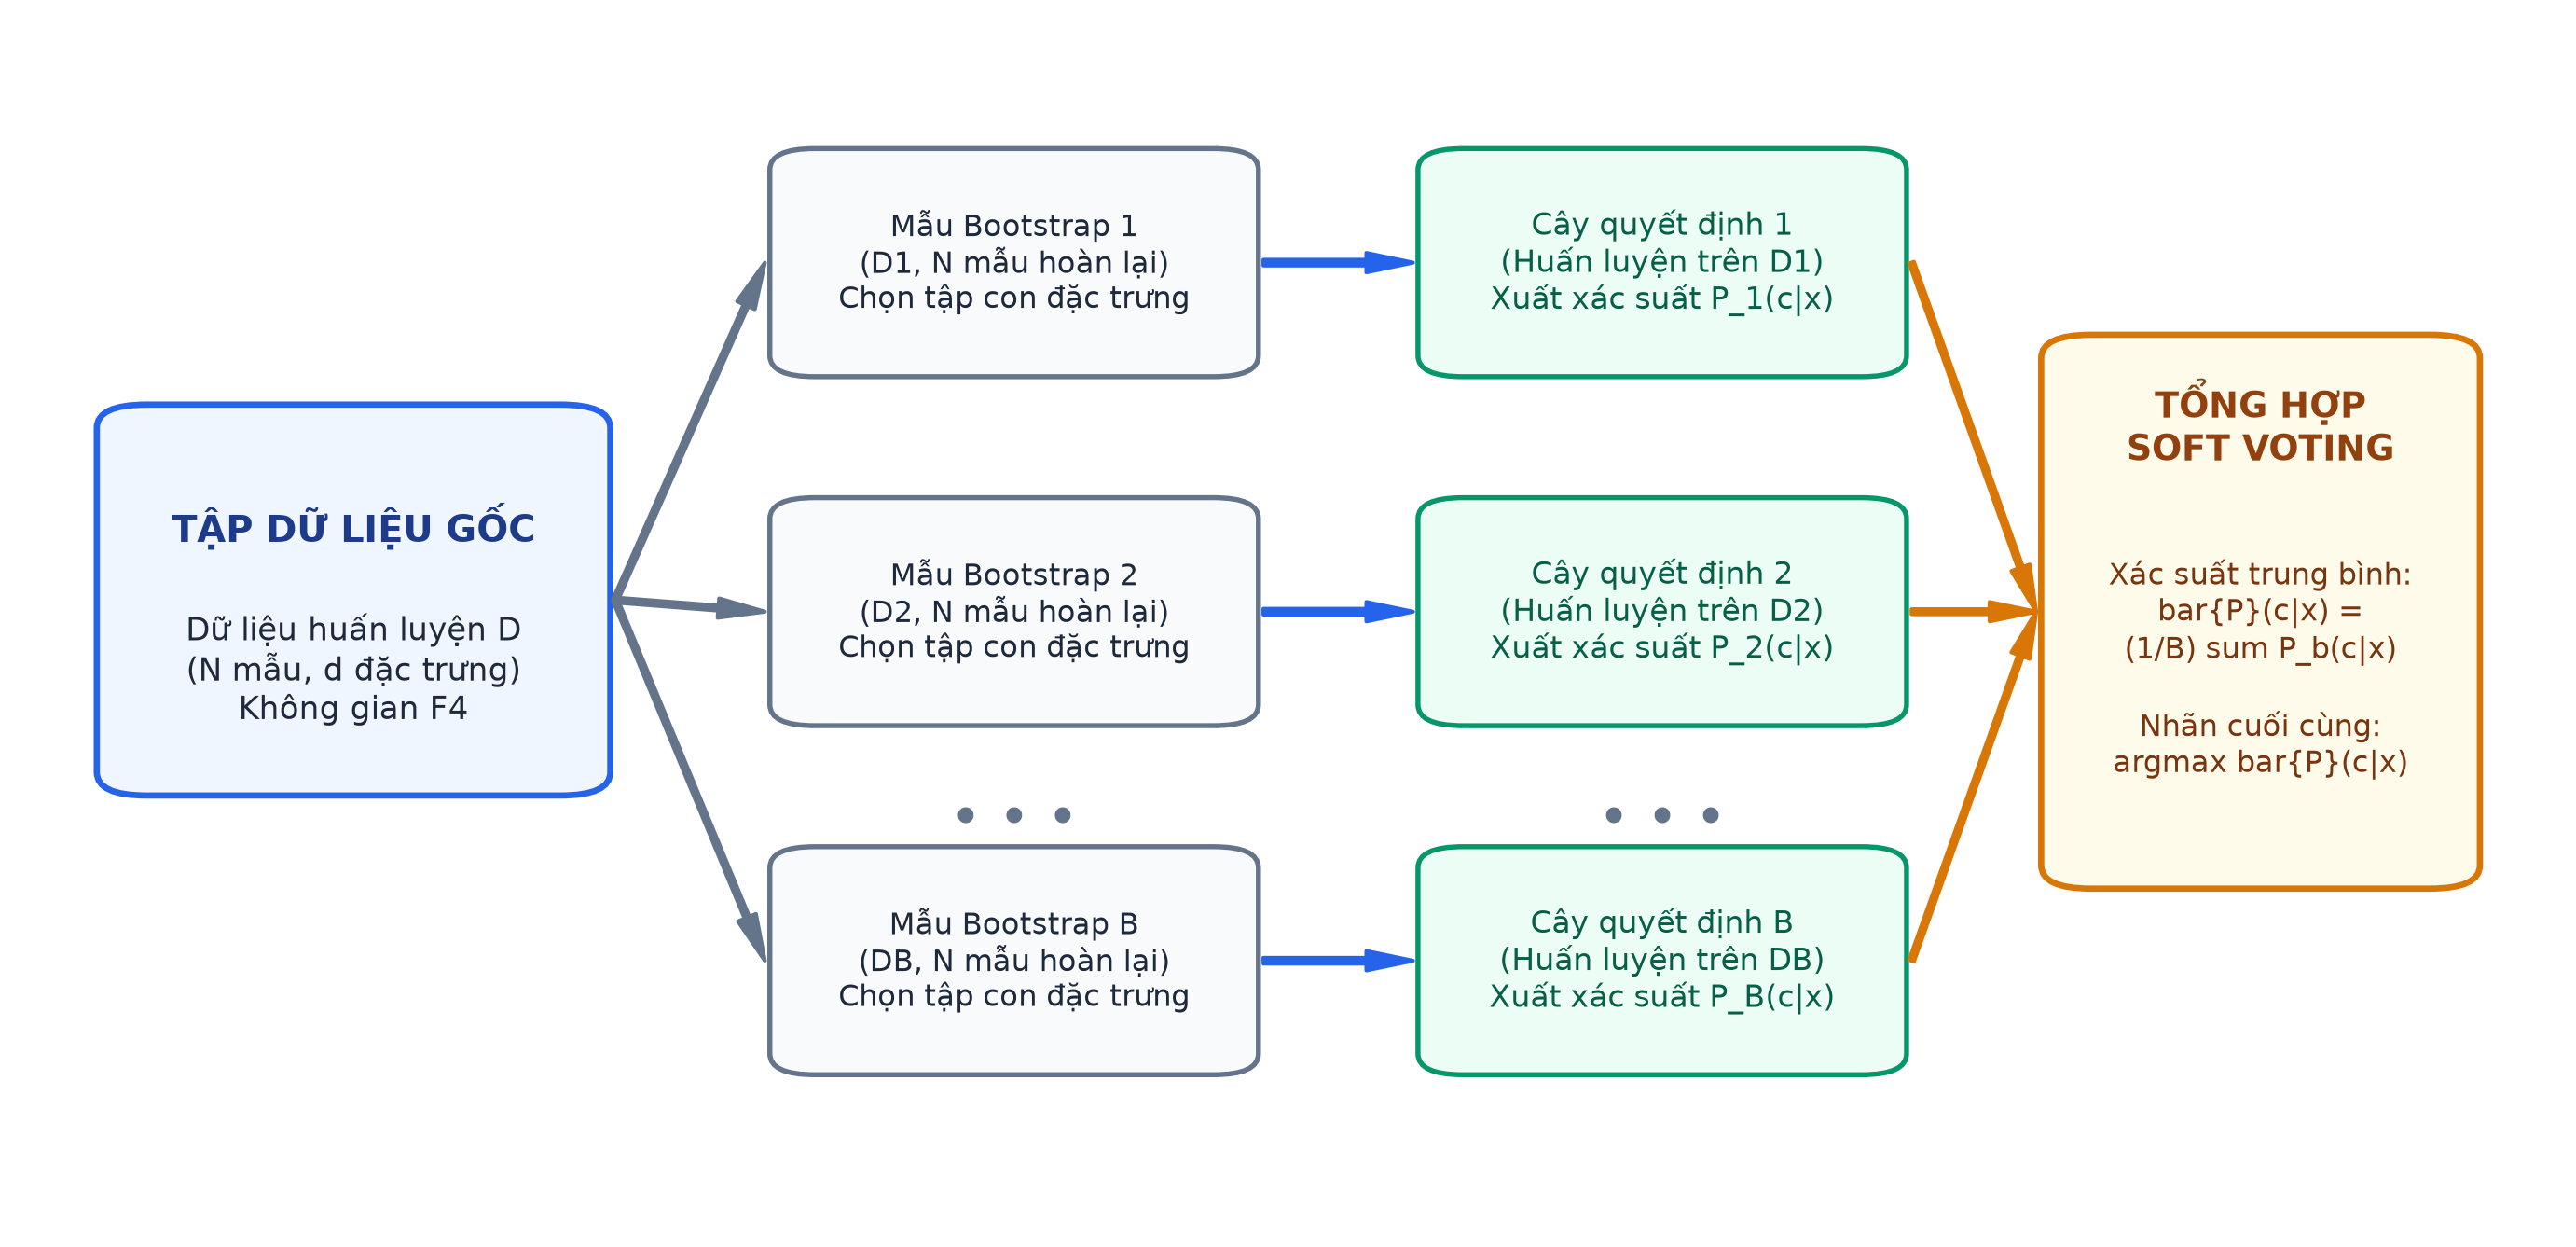
\includegraphics[width=\textwidth]{figures/fig2_random_forest_architecture.png}
\label{fig:rf-concept}
\end{figure}
\FloatBarrier

Mô hình hoạt động dựa trên ba cơ chế chặt chẽ:
\begin{enumerate}
    \item \textbf{Kỹ thuật lấy mẫu Bootstrap (Bootstrap Aggregating -- Bagging):}
    Từ tập dữ liệu huấn luyện gốc $\mathcal{D}$ gồm $N$ quan sát, thuật toán rút ngẫu nhiên có hoàn lại (sampling with replacement) đúng $N$ lần để tạo ra $B$ tập dữ liệu con độc lập $\mathcal{D}_1, \mathcal{D}_2, \dots, \mathcal{D}_B$.
    
    Về mặt lý thuyết xác suất, xác suất để một mẫu cụ thể không được chọn trong một lần rút là $1 - 1/N$. Do đó, xác suất mẫu đó không được chọn sau $N$ lần rút độc lập là:
    \begin{equation}
        \lim_{N \to \infty} \left(1 - \frac{1}{N}\right)^N = \frac{1}{e} \approx 0.368
    \end{equation}
    Điều này đồng nghĩa với việc mỗi tập dữ liệu con Bootstrap chứa khoảng $63.2\%$ số mẫu độc nhất từ tập gốc, trong khi $36.8\%$ số mẫu còn lại hoàn toàn không xuất hiện trong tập huấn luyện của cây đó và được gọi là \textbf{tập ngoài túi (Out-Of-Bag -- OOB)}. Tập OOB đóng vai trò như một tập kiểm tra độc lập tự nhiên cho từng cây mà không cần phân chia dữ liệu kiểm định trước.

    \item \textbf{Ngẫu nhiên hóa không gian đặc trưng (Random Subspace):}
    Nếu chỉ dùng Bagging đơn thuần, các cây quyết định vẫn có xu hướng chọn những đặc trưng dự báo mạnh nhất ở các nút đầu tiên, khiến cấu trúc các cây có độ tương quan cao với nhau. Để triệt tiêu độ tương quan này, tại mỗi nút rẽ nhánh của từng cây con, Random Forest chỉ cho phép thuật toán chọn ngẫu nhiên một tập con gồm $m < d$ đặc trưng (trong dự án đặt $m = 0.5 \times d$). Thuật toán chỉ tìm kiếm cặp phân tách tối ưu trên tập con $m$ đặc trưng này. Nhờ đó, các cây con được xây dựng từ những góc nhìn đặc trưng đa dạng và bổ trợ lẫn nhau.

    \item \textbf{Cơ chế giảm phương sai (Variance Reduction):}
    Tại sao việc kết hợp nhiều cây lại giúp mô hình ổn định hơn một cây đơn lẻ? Xét trung bình cộng của $B$ cây quyết định phân loại độc lập cùng phân phối, mỗi cây có phương sai dự đoán là $\sigma^2$ và hệ số tương quan trung bình giữa hai cây bất kỳ là $\rho$. Phương sai của mô hình rừng tổng hợp $\bar{f}(\mathbf{x}) = \frac{1}{B}\sum_{b=1}^B f_b(\mathbf{x})$ được biểu diễn bởi:
    \begin{equation}
        \text{Var}(\bar{f}) = \rho \sigma^2 + \frac{1 - \rho}{B} \sigma^2
    \end{equation}
    Khi số lượng cây $B$ tăng lên đủ lớn ($B \to \infty$), thành phần thứ hai $\frac{1-\rho}{B}\sigma^2$ tiệm cận về 0. Phương sai toàn thể lúc này bị chặn dưới bởi $\rho \sigma^2$. Bằng việc áp dụng ngẫu nhiên hóa đặc trưng để làm giảm mạnh hệ số tương quan $\rho$, Rừng ngẫu nhiên giảm thiểu đáng kể phương sai tổng thể so với một cây đơn lẻ ($\text{Var} \ll \sigma^2$) mà không làm tăng độ lệch (bias). Kết quả là mô hình đạt được tính ổn định và khả năng khái quát hóa vượt trội trên dữ liệu dạng bảng có nhiều nhiễu.
\end{enumerate}

\subsection{Quy trình suy luận của một mẫu dữ liệu qua Rừng ngẫu nhiên}
\label{subsec:rf-inference-pipeline}

Khi một quan sát bệnh nhân mới với vectơ đặc trưng $\mathbf{x} \in \mathbb{R}^d$ được đưa vào mô hình, quy trình dự đoán diễn ra tuần tự:
\begin{enumerate}
    \item Mẫu $\mathbf{x}$ được truyền đồng thời qua toàn bộ $B = 150$ cây quyết định đã được huấn luyện trong rừng.
    \item Tại mỗi cây $b \in \{1, \dots, B\}$, mẫu di chuyển theo các ranh giới rẽ nhánh từ nút gốc xuống nút lá. Tại nút lá đó, phân phối tỷ lệ giữa các lớp mẫu huấn luyện hình thành nên vectơ xác suất hậu nghiệm cục bộ:
    \begin{equation}
        \mathbf{p}_b(\mathbf{x}) = \left[ P_b(Y = 0 \mid \mathbf{x}), \, P_b(Y = 1 \mid \mathbf{x}), \, \dots, \, P_b(Y = K-1 \mid \mathbf{x}) \right]^T
    \end{equation}
    \item Toàn bộ rừng tổng hợp các dự đoán này thông qua cơ chế \textbf{Bỏ phiếu mềm (Soft Voting / Average Probability)}:
    \begin{equation}
        \bar{P}(Y = k \mid \mathbf{x}) = \frac{1}{B} \sum_{b=1}^B P_b(Y = k \mid \mathbf{x})
    \end{equation}
    Việc sử dụng trung bình xác suất liên tục thay vì chỉ bỏ phiếu cứng (Hard Voting -- đếm số phiếu của lớp chiếm đa số) giúp bảo toàn mức độ tự tin định lượng của từng cây con, tạo ra phân phối xác suất trơn mượt phục vụ trực tiếp cho các cơ chế định tuyến phân cấp và đánh giá rủi ro nhạy chi phí Bayes tiếp theo.
    \item Quyết định phân loại cuối cùng trong mô hình phẳng được xác định bằng lớp có xác suất trung bình cực đại: $\hat{y} = \arg\max_k \bar{P}(Y = k \mid \mathbf{x})$.
\end{enumerate}

\subsection{Vai trò của các siêu tham số Random Forest trong dự án DepSev-ML}
\label{subsec:rf-hyperparameters-role}

Trong dự án DepSev-ML, cấu hình Rừng ngẫu nhiên tối ưu được xác lập qua quy trình Nested CV và cố định thành \textbf{Frozen Random Forest Spec} với các siêu tham số mang ý nghĩa thực tiễn rõ rệt:
\begin{itemize}
    \item \texttt{n\_estimators = 150}: Số lượng cây trong rừng. Giá trị $B = 150$ đủ lớn để phương sai hội tụ ổn định, đảm bảo sai số xấp xỉ xác suất qua Soft Voting ở mức tối thiểu mà không gây lãng phí bộ nhớ và thời gian tính toán.
    \item \texttt{max\_depth = 8}: Giới hạn độ sâu tối đa của từng cây. Dữ liệu cận lâm sàng chứa nhiều nhiễu ngẫu nhiên; việc khống chế độ sâu ở mức 8 ngăn ngừa việc cây rẽ nhánh quá sâu để cố gắng khớp các mẫu ngoại lai (outliers), kiểm soát chặt chẽ hiện tượng quá khớp.
    \item \texttt{max\_features = 0.5}: Tỷ lệ đặc trưng ngẫu nhiên được chọn tại mỗi nút rẽ nhánh. Với không gian 34 biến ($F_4$), mỗi nút chỉ xem xét ngẫu nhiên $17$ đặc trưng, giúp giải tương quan mạnh mẽ giữa các cây trong quần thể rừng.
    \item \texttt{min\_samples\_split = 10} và \texttt{min\_samples\_leaf = 8}: Tiêu chuẩn kích thước mẫu tối thiểu. Một nút chỉ được phân tách nếu chứa ít nhất 10 mẫu, và mỗi nút lá phải đại diện cho tối thiểu 8 quan sát. Ràng buộc này bảo đảm phân phối xác suất tại nút lá có ý nghĩa thống kê và loại bỏ các nút lá cá biệt.
    \item \texttt{class\_weight = 'balanced\_subsample'}: Cơ chế điều chỉnh trọng số nghịch đảo tần số lớp trên từng mẫu bootstrap riêng biệt:
    \begin{equation}
        w_k^{(b)} = \frac{N^{(b)}}{K \cdot N_k^{(b)}}
    \end{equation}
    Đối với dữ liệu y tế mất cân bằng trầm trọng như NHANES (tỷ số mất cân bằng $68.5:1$), kỹ thuật này buộc từng cây quyết định phải gia tăng mức phạt khi phân loại sai các ca bệnh hiếm thuộc nhóm triệu chứng nặng ($C_3, C_4$), cải thiện độ nhạy mà không cần can thiệp nhân tạo vào phân phối mẫu gốc.
\end{itemize}

Quy trình triển khai từng bước thuật toán Random Forest trên dữ liệu thực tế NHANES cùng nguyên tắc chống rò rỉ thông tin tuyệt đối (Zero Data Leakage) sẽ được mô tả chi tiết tại Mục \ref{sec:xay-dung-random-forest} (Chương \ref{ch:phuong-phap}); các kết quả định lượng, ma trận nhầm lẫn 5 lớp và giới hạn lâm sàng của mô hình sẽ được phân tích sâu trong Chương \ref{ch:thuc-nghiem}.

\section{Các trường phái mô hình hóa trong bài toán phân loại thứ bậc}
\label{sec:truong-phai-mo-hinh-hoa}

Để xử lý bài toán phân tầng nguy cơ trầm cảm, nghiên cứu khảo sát và so sánh ba trường phái mô hình hóa chính được minh họa trong Hình \ref{fig:modeling-paradigms}.

\begin{figure}[htbp]{Ba trường phái mô hình hóa: (a) Phân loại phẳng, (b) Phân loại phân cấp hai giai đoạn, và (c) Phân loại thứ bậc}
\centering
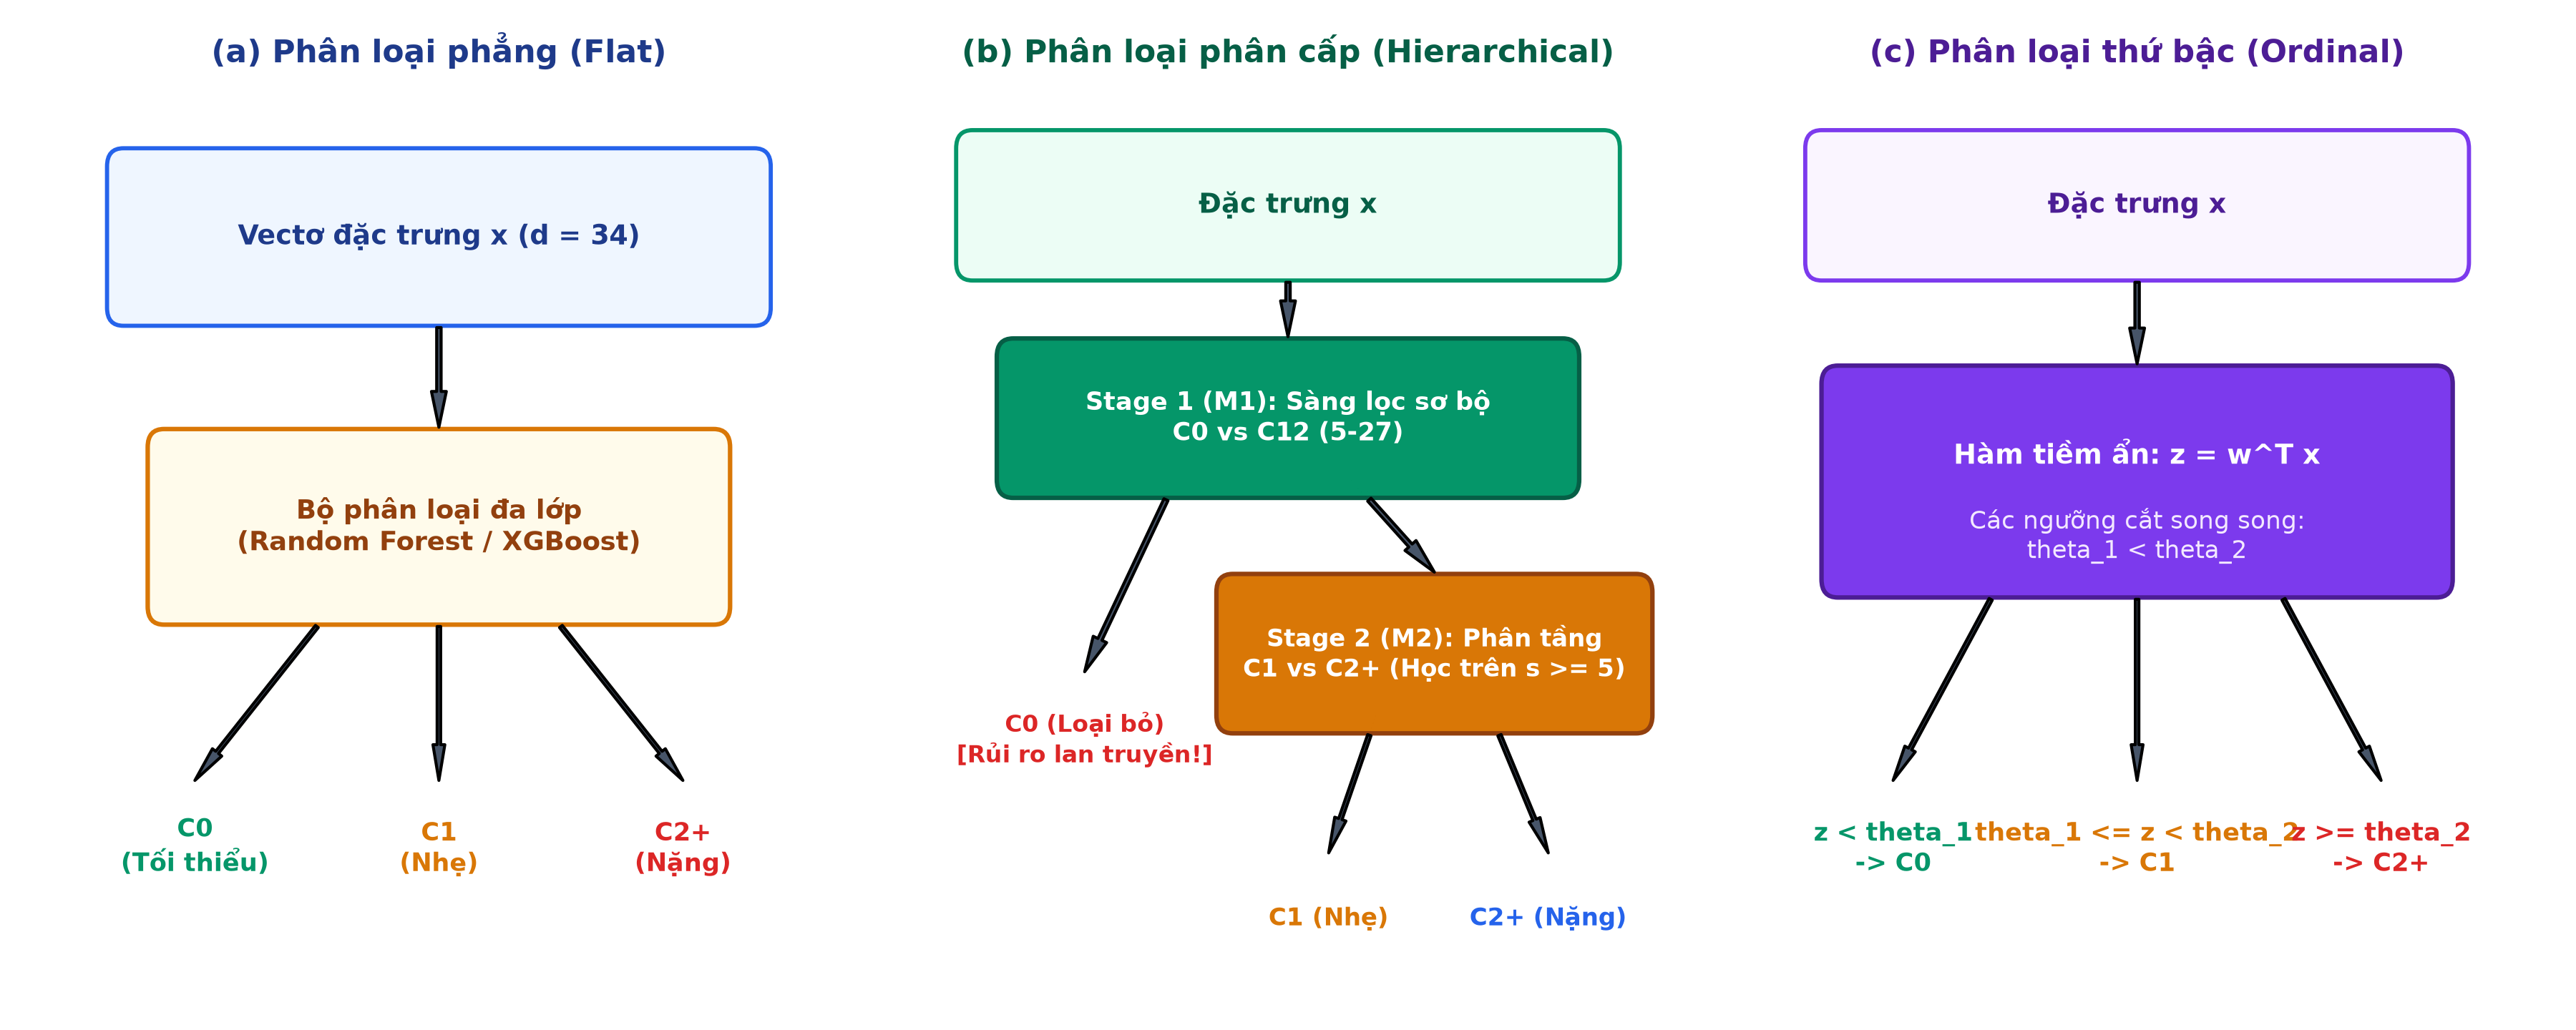
\includegraphics[width=\textwidth]{figures/fig2_modeling_paradigms.png}
\label{fig:modeling-paradigms}
\end{figure}
\FloatBarrier

\subsection{Trường phái phân loại phẳng (Flat Classification)}
\label{subsec:flat-paradigm}

Cách tiếp cận phân loại phẳng coi $K$ mức độ nghiêm trọng là các nhãn danh nghĩa hoàn toàn độc lập. Mô hình học trực tiếp một hàm ánh xạ $f: \mathbb{R}^d \to \Delta^K$ để dự đoán phân phối xác suất hậu nghiệm $P(Y = k \mid \mathbf{x})$. Các thuật toán cơ sở bao gồm Hồi quy Logistic đa thức, Rừng ngẫu nhiên (Random Forest) và XGBoost.

Hạn chế căn bản của trường phái phân loại phẳng là bỏ qua hoàn toàn quan hệ thứ bậc tự nhiên giữa các mức độ ($C_0 < C_1 < C_2$). Một sai lầm nhầm lẫn giữa $C_0$ và $C_1$ (cách nhau 1 bậc) bị hàm mất mát đối xử tương đương như sai lầm cực kỳ nguy hiểm giữa $C_0$ và $C_2^+$ (cách nhau 2 bậc). Đồng thời, khi dữ liệu bị mất cân bằng trầm trọng, các ranh giới phân tách phẳng dễ bị đẩy ép về phía các lớp thiểu số.

\subsection{Trường phái phân loại phân cấp (Hierarchical Classification)}
\label{subsec:hierarchical-paradigm}

Nhằm mô phỏng quy trình sàng lọc lâm sàng thực tế của bác sĩ (trước hết xác định người đó có triệu chứng hay không, sau đó mới đánh giá mức độ nặng), trường phái phân cấp chia nhỏ bài toán phức tạp thành một cấu trúc cây gồm hai giai đoạn \cite{silla2011survey}:
\begin{itemize}
    \item \textbf{Giai đoạn 1 (Bộ phân loại sàng lọc $M_1$):} Phân loại nhị phân giữa nhóm không có triệu chứng ($C_0$) và nhóm có triệu chứng ($C_{12} = C_1 \cup C_2^+$).
    \item \textbf{Giai đoạn 2 (Bộ phân loại phân tầng $M_2$):} Tiếp nhận các đối tượng được xác định có triệu chứng để phân biệt giữa mức độ nhẹ ($C_1$) và mức độ nặng ($C_2^+$).
\end{itemize}

Kiến trúc phân cấp chia làm hai cơ chế định tuyến:
\begin{enumerate}
    \item \textbf{Định tuyến cứng (Hard Routing):} Nếu $M_1$ dự đoán một mẫu là $C_0$, mẫu đó lập tức bị loại bỏ khỏi luồng xử lý và không bao giờ được $M_2$ xem xét. Cơ chế này dẫn đến hiện tượng \textbf{lan truyền sai số một chiều (Error Propagation)}: nếu một ca bệnh nặng $C_2^+$ bị $M_1$ gán nhầm thành $C_0$, sai sót này sẽ bị khóa vĩnh viễn và biến thành lỗi nghiêm trọng nhất trong y khoa.
    \item \textbf{Định tuyến mềm (Soft Routing):} Cả hai mô hình $M_1$ và $M_2$ đều xuất ra xác suất liên tục. Xác suất hậu nghiệm toàn thể được tính bằng công thức xác suất toàn phần:
    \begin{align}
        \hat{P}(C_0 \mid \mathbf{x}) &= P_{M_1}(C_0 \mid \mathbf{x}) \\
        \hat{P}(C_1 \mid \mathbf{x}) &= P_{M_1}(C_{12} \mid \mathbf{x}) \cdot P_{M_2}(C_1 \mid C_{12}, \mathbf{x}) \\
        \hat{P}(C_2^+ \mid \mathbf{x}) &= P_{M_1}(C_{12} \mid \mathbf{x}) \cdot P_{M_2}(C_2^+ \mid C_{12}, \mathbf{x})
    \end{align}
    Cơ chế mềm bảo toàn thông tin xác suất liên tục và loại bỏ hoàn toàn hiện tượng nghẽn sai số của định tuyến cứng.
\end{enumerate}

\subsection{Lý thuyết quyết định nhạy chi phí Bayes (Bayes Cost-Sensitive Decision)}
\label{subsec:cost-sensitive-paradigm}

Trong sàng lọc y tế, các loại sai lầm không có hậu quả ngang nhau: việc bỏ sót một ca bệnh nặng ($C_2^+ \to C_0$) nguy hiểm hơn rất nhiều so với một ca báo động nhầm ($C_0 \to C_2^+$). Lý thuyết quyết định nhạy chi phí Bayes \cite{elkan2001foundations} cung cấp cơ sở toán học để tối ưu hóa quyết định dưới sự bất cân xứng này.

Cho ma trận chi phí $\mathbf{C} \in \mathbb{R}^{K \times K}$, trong đó $\mathbf{C}(i, j)$ là chi phí khi dự đoán lớp $i$ trong khi nhãn thực tế là $j$ (với $\mathbf{C}(i, i) = 0$). Quy tắc quyết định tối ưu Bayes là chọn nhãn $\hat{y}^*$ sao cho tối thiểu hóa rủi ro kỳ vọng:
\begin{equation}
    \hat{y}^* = \arg\min_{i \in \{0, \dots, K-1\}} \sum_{j=0}^{K-1} \mathbf{C}(i, j) \hat{P}(C_j \mid \mathbf{x})
\end{equation}
Bằng cách gán trọng số phạt nặng cho phần tử $\mathbf{C}(0, 2)$, mô hình chủ động dịch chuyển ranh giới quyết định để bảo vệ nhóm bệnh nhân nặng, tạo ra sự đánh đổi lâm sàng minh bạch và có thể kiểm soát.

\subsection{Trường phái phân loại thứ bậc (Ordinal Classification)}
\label{subsec:ordinal-paradigm}

Do các mức độ triệu chứng PHQ-9 có tính chất thứ bậc tự nhiên ($C_0 < C_1 < C_2$), phân loại thứ bậc khai thác cấu trúc trật tự này để hạn chế các sai số nhảy bậc lớn \cite{mccullagh1980regression, frank2001simple}:
\begin{enumerate}
    \item \textbf{Mô hình Hồi quy Logistic thứ bậc (Ordinal Logistic Regression -- OLR):} Giả định tồn tại một biến trạng thái tiềm ẩn tuyến tính $z = \mathbf{w}^T \mathbf{x}$ và tập hợp các ngưỡng cắt đơn điệu $\theta_1 < \theta_2 < \dots < \theta_{K-1}$. Xác suất tích lũy được mô hình hóa theo hàm phân phối Logistic:
    \begin{equation}
        P(Y \le k \mid \mathbf{x}) = \sigma(\theta_{k+1} - \mathbf{w}^T \mathbf{x}) = \frac{1}{1 + e^{-(\theta_{k+1} - \mathbf{w}^T \mathbf{x})}}
    \end{equation}
    Mô hình OLR sử dụng chung một vectơ trọng số $\mathbf{w}$ cho tất cả các ranh giới (giả định tỷ lệ chênh tỉ lệ thuận -- proportional odds), giúp số lượng tham số tinh gọn và tự động bảo đảm các mặt siêu phẳng quyết định song song không bao giờ cắt nhau.
    \item \textbf{Phân loại nhị phân tích lũy (Cumulative Binary Classification -- CBC):} Huấn luyện $K-1$ bộ phân loại nhị phân độc lập $h_k(\mathbf{x})$ để dự đoán biến cố tích lũy $P(Y \ge k \mid \mathbf{x})$. Tuy nhiên, phương pháp này tiềm ẩn nguy cơ \textbf{vi phạm tính đơn điệu xác suất} khi một điểm dữ liệu xuất hiện tình huống $P(Y \ge k+1) > P(Y \ge k)$.
\end{enumerate}

\section{Tổng quan các nghiên cứu liên quan}
\label{sec:nghien-cuu-lien-quan}

Trong thập kỷ qua, việc ứng dụng học máy vào dữ liệu sức khỏe cộng đồng NHANES để nghiên cứu bệnh trầm cảm đã thu hút nhiều sự quan tâm. Bảng \ref{tab:related-works} tổng hợp các công trình tiêu biểu trong y văn.

\begin{table}{Tổng hợp so sánh các nghiên cứu liên quan về dự đoán trầm cảm từ dữ liệu y tế}
\centering
\footnotesize
\setlength{\tabcolsep}{3pt}
\label{tab:related-works}
\begin{tabularx}{\textwidth}{p{3.2cm} p{2.2cm} p{2.4cm} p{2.8cm} X}
\toprule
\textbf{Nghiên cứu} & \textbf{Nguồn dữ liệu} & \textbf{Không gian đích} & \textbf{Phương pháp học máy} & \textbf{Hạn chế chính} \\
\midrule
Pratt và cộng sự (2014) \cite{pratt1991discriminant} & NHANES 2009--2012 & Nhị phân ($s \ge 10$) & Thống kê dịch tễ mô tả, Hồi quy đa biến & Chỉ phân tích tương quan đơn biến, không xây dựng mô hình dự đoán \\
\midrule
Patel và cộng sự (2016) & NHANES đa chu kỳ & Nhị phân ($s \ge 10$) & Logistic Regression, Cây quyết định & Chỉ làm nhị phân $T_2$, không phân tầng đa mức độ nghiêm trọng \\
\midrule
Dipnall và cộng sự (2016) & Dữ liệu lâm sàng & Nhị phân ($s \ge 10$) & Khai phá chỉ dấu sinh học, PCA, GLM & Thiếu quy trình kiểm định chéo lồng nhau nghiêm ngặt, rủi ro rò rỉ \\
\midrule
Zhang và cộng sự (2020) & Khảo sát cộng đồng & Đa lớp (3 mức) & Random Forest, XGBoost phẳng & Bỏ qua quan hệ thứ bậc, tỷ lệ bỏ sót ca nặng rất cao \\
\midrule
Kaggle Benchmark CDC (2021) & NHANES 2013--2014 & Nhị phân / 5 lớp & Baseline Ensembles, Deep ANN & Đánh giá thiên lệch qua Accuracy, không phân tích đánh đổi chi phí \\
\midrule
\textbf{DepSev-ML (Báo cáo này)} & \textbf{NHANES 3 chu kỳ (2011--2016)} & \textbf{Đa mức độ ($T_2, T_3, T_4, T_5$)} & \textbf{Phân cấp mềm, Quyết định Bayes, Phân loại thứ bậc} & \textbf{Giải quyết toàn diện mất cân bằng, đánh đổi lâm sàng và kiểm định trôi phân phối} \\
\bottomrule
\end{tabularx}
\end{table}

Qua khảo sát y văn, có thể rút ra ba khoảng trống nghiên cứu chính:
\begin{enumerate}
    \item Phần lớn các nghiên cứu chỉ dừng lại ở bài toán nhị phân thô ($s \ge 10$ hoặc $s \ge 5$). Rất ít công trình khảo sát quy luật suy giảm hiệu năng khi mở rộng sang không gian đa lớp chi tiết ($T_3 \to T_5$).
    \item Các nghiên cứu đa lớp hiện có chủ yếu áp dụng mô hình phân loại phẳng truyền thống, bỏ qua quan hệ thứ bậc và không đo lường hệ quả của việc bỏ sót ca nặng theo góc nhìn y tế thực tế.
    \item Chưa có công trình nào đánh giá có hệ thống sự khác biệt giữa phân cấp cứng và phân cấp mềm kết hợp tối ưu chi phí Bayes, cũng như kiểm tra độ bền vững của mô hình trên tập kiểm tra ngoại suy độc lập theo dòng thời gian.
\end{enumerate}

\section{Tóm tắt chương}
\label{sec:tom-tat-chuong-2}

Chương 2 đã thiết lập nền tảng lý thuyết vững chắc cho nghiên cứu thông qua việc làm rõ thang đo PHQ-9, cơ sở sinh học kết nối các chỉ số xét nghiệm với triệu chứng tâm thần, và bản chất hình học của hai thách thức lớn: mất cân bằng lớp cực đoan và chồng lấn đặc trưng sinh lý. Chương cũng đã phân tích ưu nhược điểm của ba trường phái mô hình hóa (phẳng, phân cấp, thứ bậc) và định vị rõ khoảng trống học thuật cần giải quyết. Các phân tích này là cơ sở trực tiếp để xây dựng khung thực nghiệm DepSev-ML được trình bày chi tiết trong Chương \ref{ch:phuong-phap}.

